\chapter{Synthesis as a Game}

In the following sections we formalise the device driver synthesis problem using games. We show that GR(1) games are sufficient to capture the properties of the drivers that we require.

We formalize the driver synthesis problem as a \emph{two-player game}~\cite{Thomas_95} between the driver and its environment. The game is played over a finite automaton that represents all possible states and behaviors of the system. Transitions of the automaton are classified into \emph{controllable} transitions triggered by the driver and \emph{uncontrollable} transitions triggered by the device or OS. A winning strategy for the driver in the game corresponds to a correct driver implementation. If, on the other hand, a winning strategy does not exist, this means that there exists no specification-conforming driver implementation.

Two-player games naturally capture the essence of the driver synthesis problem: the driver must enforce a certain subset of system behaviors while having only partial control over the system. The game-based approach leads to a precise mathematical formulation of the problem and enables us to apply theoretical results and algorithms from game theory to driver synthesis.

Figure~\ref{f:game} illustrates the concept using a trivial game automaton that models the core of our running example. Controllable and uncontrollable transitions of the automaton are shown with solid and dashed arrows respectively.  The goal of the driver in the game is to infinitely often visit the initial state, labelled \src{G}, which represents the situation when the driver does not have any outstanding requests.  After getting a \src{send} request from the OS, the driver must write data and command registers to start the data transfer.  Writing the command register first may trigger a hardware send event before the driver has a chance to write the data register.  As a result, wrong data value gets sent, taking the game into an error state \src{E}.  Hence, state $s_4$ is losing for the driver.  To avoid this state, the correct strategy for the driver is to play \src{write\_data} in state $s_2$, followed by \src{write\_cmd}.  In $s_5$ the driver must remain idle until the environment executes the \src{evt\_send} transition.

\begin{figure}[t]
    \center
    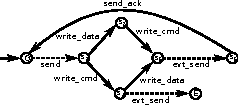
\includegraphics[width=0.7\linewidth]{imgs/game.pdf}
    \caption{A simple two-player game.}
    \label{f:game}
\end{figure}

\section{The Players}

To formalise the driver synthesis problem using games, the first thing we must define is the players:

\begin{itemize}
    \item Player~1 is the driver. 
    \item Player~2 is the environment, which consists of the device to be controlled as well as the operating system.
\end{itemize}

\section{GR(1) based formalism}

In the following sections, we attempt to formalise the driver synthesis problem using the simplest game - the reachability game - and analyse its shortcomings. We show that extending our formalism to GR(1) objectives, as used in Termite, overcomes these shortcomings.

\subsection{Reachability}

As a concrete example, we could create a crude formalism for driver synthesis using only a reachability game. Consider, for example, figure~\ref{fig:reach}, which shows the state machine for a game to control a hypothetical network controller. Execution begins in the leftmost state where the OS may initiate a network transfer by choosing the `send' label. The goal of the game is the rightmost state (labelled `G' and with a double circle) as this is the point where player 1 has completed the request. So, to win, player 1 (who controls the transitions with solid lines) must ensure that execution of the state machine reaches the goal. 

\begin{figure}
\centering
\includegraphics[width=0.85\linewidth]{diagrams/reachGame.pdf}
\caption{Reachability game for simple network device}
\label{fig:reach}
\end{figure}

The network device has two 8-bit registers, command (abbreviated cmd) and data. Writing 0x01 to the command register starts the transfer, and eventually whatever is in the data register gets written out to the network. Note that the actual sending of the data is an uncontrollable event. 

The correct sequence to win the game, therefore, is to write to the data register and then to the control register after the OS performs a send request. This takes us to state `S5' where the only move by player 2 is `evt\_send' taking us to the goal. 

If the command register is written first and then the data register there is potential for the environment to play the `evt\_send' label before the data is written, potentially resulting in the wrong data being sent. This is the transition that terminates in the `E' state (for error). The `E' state is a dead end, so it is not possible to reach the goal. 

So, if player 1 takes the top half of the diamond (i.e.\ writes data before command) then it will be guaranteed to reach the goal and the reachability game is winning for player 1. The strategy to reach the goal tells us the sequence of labels the driver must play to get to the goal. In principle, this could be turned into a driver for our simple network device.

This simplistic formalism for driver synthesis has several shortcomings that we will deal with in the following sections.

\subsection{\buchi}

Consider a simplified version of the previous network controller that does not have a command register. Instead, writing to the data register triggers future transmission of the byte. However, there are two ways of writing to the data register. One is a standard register write. The other also performs the register write and then schedules a self destruct sequence to happen immediately after the byte is transmitted. The state machine for this device is shown in figure~\ref{fig:buchi}. The goal, in this case, is the set $\{S3, S5\}$ corresponding to the state after completion of the send request. The problem is that, unless you only ever want to send one byte, this goal does not capture the required behavior. For example, a valid strategy for the reachability game with objective $\{S3, S5\}$ is to take the bottom branch of the specification, putting the device in a state where it is not possible to transmit another packet. One could easily work around this problem by specifying only ${S3}$ as the goal, but this breaks composition of the specifications (Section~\ref{sec:composition}).

The solution is to modify the objective of the game. Instead of being able to reach the goal once, we want to be able to reach the goal an infinite number of times. Or, equivalently, we want to always be able to reach the goal again. This is a \buchi\ game.

\begin{figure}
\centering
\includegraphics[width=0.85\linewidth]{diagrams/buchiGame.pdf}
\caption{\buchi\ game for the simple network device}
\label{fig:buchi}
\end{figure}

\subsection{Fairness}

Consider another modification of our simplified network device without a self destruct sequence, but with the ability to check that noone is using the communication medium prior to transmitting. The state machine of this device is given in figure~\ref{fig:fair}. After the user requests data transmission by writing to the data register, it executes a loop that checks if the medium is free, and if so, it performs the transmission. 

If we pose this as a reachability game with goal state $G$, then the game is not winnable. The device may stay in the loop forever as it is never guaranteed to exit. Such a behavior should not prevent a driver from being synthesized providing that we have good reason to believe that the loop will eventually exit. Looping forever can be seen as a invalid behavior and we want to synthesize a driver for this system providing the invalid behavior does not occur. 

These behaviors are eliminated with fairness conditions (Section~\ref{sec:fairness}). Fairness conditions are sets of states which we guarantee execution will eventually leave. We refer to these as unfair states. In the example, the unfair states are the set $\{S2, S3\}$. The fairness condition says that we will eventually leave the unfair set once we enter it, and the only way of doing this is through the $evt\_send$ transition, so the game becomes winning.

\begin{figure}[t]
\centering
\includegraphics[width=0.85\linewidth]{diagrams/fairReach.pdf}
\caption{Fair reachability game for the simple network device}
\label{fig:fair}
\end{figure}

\subsection{GR(1)}

We allow multiple goals as real drivers may be required to meet multiple objectives. Additionally, we allow multiple fairness conditions as real drivers may have multiple `looping' behaviors that need to be ruled out.

The combination of multiple fairness and multiple \buchi\ objectives is a GR(1) objective (Section~\ref{sec:gr1}). Intuitively a GR(1) objective says that we can always reach any goal provided that we do not get stuck forever in some unfair set of states. We use GR(1) objectives in Termite as we have found that in practice they are sufficient to express the requirements of our drivers.

\section{Device and OS specifications and synchronization}
\label{sec:composition}

A core concept of Termite is the separation of device and operating system specifications. This allows us to reuse the same device specification with different OS specifications as well as reusing the same OS specification with different devices. Games so far have been defined to have a single state machine that contains all of the states of the system as well as all of the actions. In Termite, we decouple the description of the operating system from the device to be controlled and then combine these to form a state machine before synthesis.

Both the device and OS specifications are given as state machines. In Termite, they are defined symbolically in TSL (Termite specification language) (Appendix~\ref{ch:tsl_ref}). Each specification has its own set of state variables that it must supply update functions for. There is also a global set of label variables which each specification may also refer to in its state update functions. The actual update functions are provided by the TSL compiler which generates them from a high level C-like language. In this section, we work at the level of state machines and not the TSL they are generated from.

We give an example system specification to illustrate its decomposition into separate OS and device specifications. 

\subsection{State Machines}

Figure~\ref{fig:dev_spec} is our example device specification. The labelled circles are states. Arrows represent transitions between states. Solid arrows are controllable transitions whereas dashed arrows are uncontrollable, as described in Section~\ref{sec:termite_cpre}. Each transition is labelled by at least one event. Conceptually, these events trigger the transitions. All events for which there are no outgoing transitions do not change the state, i.e.\ they are self loops and are not shown in the interest of keeping the diagrams concise. The short arrow with no source state indicates the initial state. There may be more than one initial state, in which case the initial state is chosen non-deterministically by the environment.

\subsection{Device Specification}

We start with the device specification given in Figure~\ref{fig:dev_spec}. Our device is a hypothetical trivial UART-like device. Instead of sending bytes, it sends notifications, which carry no value. Its programming interface consists of an action, \code{devSendReq}, that requests that the device send a notification. In a real system this could be a write to a particular bit in a control register that triggers the device action. This action only has an effect in the \code{devIdle} state and it causes the device to transition to the \code{devSending} state. From there, when the \code{devSent} event happens, which corresponds to the device actually sending the notification, the device transitions back to the \code{devIdle} state. Additionally, it emits the \code{classSent} event. We will respond to the \code{classSent} event in the OS specification in the next section. From here, another notification may be requested by performing the \code{devSendReq} action again.

This device model is equivalent to a Mealy machine as shown in Figure~\ref{fig:dev_spec_mealy}. There is a single register for storing the current state and this state is updated on each transition using logic which additionally takes the label variables as input. This logic also produces the output boolean variable \code{classSent}.

\begin{figure}
\centering
\begin{subfigure}[t]{0.47\textwidth}
\includegraphics[width=\linewidth]{diagrams/exampleSpecDevice.pdf}
\caption{Device specification}
\label{fig:dev_spec}
\end{subfigure}
\hfill
\begin{subfigure}[t]{0.47\textwidth}
\includegraphics[width=\linewidth]{diagrams/devMealy.pdf}
\caption{Device specification}
\label{fig:dev_spec_mealy}
\end{subfigure}
\end{figure}

\subsection{OS specification}

\begin{figure}
\centering
\begin{subfigure}[t]{0.47\textwidth}
\includegraphics[width=\linewidth]{diagrams/exampleSpecOS.pdf}
\caption{OS specification}
\label{fig:os_spec}
\end{subfigure}
\hfill
\begin{subfigure}[t]{0.47\textwidth}
\centering
\includegraphics[width=\linewidth]{diagrams/osMealy.pdf}
\caption{OS specification}
\label{fig:os_spec_mealy}
\end{subfigure}
\end{figure}

The operating system specification, given in Figure~\ref{fig:os_spec} is like a test harness for our driver. It specifies which requests the driver may receive (e.g.\ to send a notification) and how it must respond (e.g.\ by eventually sending the requested notification). It is simply another state machine, like the device specification, but it may also have goals.

The goal state, state \code{O2}, is the state that a correct driver will eventually force the OS specification to be in. It is possible to specify multiple goal states, in which case the driver must force execution into any goal state.

Our OS state machine starts off in the \code{osIdle} state. From there, if a \code{classSent} event is triggered by the device state machine, then the device must have sent a notification without the OS ever having requested one. This is an error, so the OS state machine transitions to the \code{osError} state. There is no way that the OS could have known that this event happened as it does not monitor the device notification output, so, the OS specification does not represent the way that the OS behaves in reality. These events that do not correspond to real interactions but are used to enforce correctness are called \emph{virtual events}. Responding to virtual events in this way is how the OS spec guarantees correctness of the system. 

There is nothing special about the error state, however, we have constructed the state machine in such a way that the error state is a dead end and it is not possible to reach the goal from that state.

If a \code{devSndReq} event happens, the OS transitions into the \code{devRequested} state. From there, when a \code{classSent} event happens, the OS specification transitions into the goal state as this time the \code{classSent} event was expected. 

We can see from the OS specification that it is the job of the driver to ensure that a \code{devSendReq} event is eventually followed by \code{classSent} event. However, a \code{classSent} event can only be issued by the device, not the driver. The driver can, however, force the device to issue a \code{classSent} event indirectly in response to a \code{devSendReq} event. 

In general, it is the job of the driver synthesis algorithm to figure out how to force certain events to happen at the right time (as specified by the OS state machine) by using information from the device state machine. 

As with the device specification, the OS specification may be seen as a Mealy machine as shown in Figure~\ref{fig:os_spec_mealy}. Again, there is a single register for storing the current state and this state is updated on each transition using combinational logic. In addition to taking the label variables as input, it also takes the \code{classSent} boolean signal that was produced by the device Mealy machine as input. 

\subsection{Combined Specification}

We combine the device and OS specifications by executing them concurrently. We do this by instantiating both Mealy machines in parallel and connecting the signals, as shown in Figure~\ref{fig:combined_spec_mealy}. Figure~\ref{fig:combined_spec} shows the state machine of the combined specification. This cumbersome state machine shows the size and complexity advantages of using separate Mealy machines in parallel as the specification language. A state is a goal state if the state that it corresponds to in the OS or device state machine is a goal state. Both of the states on the right of Figure~\ref{fig:combined_spec} correspond to state \code{O2} in the OS specification, which is a goal, so they are goals. It is possible to have goals in the device specification but they are not useful in practice. Fair regions work in the same way.

\begin{figure}
\centering
\begin{subfigure}[t]{0.47\textwidth}
\includegraphics[width=\linewidth]{diagrams/exampleSpecCombined.pdf}
\caption{Combined specification}
\label{fig:combined_spec}
\end{subfigure}
\hfill
\begin{subfigure}[t]{0.47\textwidth}
\includegraphics[width=\linewidth]{diagrams/combinedMealy.pdf}
\caption{Combined specification}
\label{fig:combined_spec_mealy}
\end{subfigure}
\end{figure}

